%
% Clases de módulo DRBG
% Análisis y diseño de programa tokenizador, reporte técnico.
%
% Proyecto Lovelace.
%

\subsection{Clases de \texorpdfstring{\acrshort{gl:drbg}}{DRBG}}
\label{sec:drbg_disenio}

Las clases relacionadas con el generador de números pseudoaleatorio se muestran
en la figura~\ref{clases_drbg}. Nuevamente, todas las clases pertenecen al
paquete de las implementaciones.

Un \gls{gl:drbg} implementa la interfaz de una función que recibe enteros sin
signo y entrega arreglos de bytes. Esta clase define la estructura general de un
generador: las cinco funciones definidas por el estándar del NIST (ver sección
\ref{sec:generadores_pseudoaleatorios}) y el conjunto de valores miembro que
conforman el estado del generador. El \gls{gl:drbg} declara la función abstracta
para generar bytes; todos los posibles generadores concretos deben implementar
esta función para poder tener un generador completo.

La clase del generador necesita una fuente de entropía (o fuente de
aleatoriedad). Siguiendo el esquema de débil acomplamiento dado por las
interfaces de las funciones, la fuente de entropia es una función que recibe un
entero y regresa un arreglo de bytes. En el costado izquierdo del diagrama se
muestran dos de las posibles fuentes de entropia: aleatoriedad trivial y
aleatoriedad por hardware (para más detalles, ver sección~\ref{sec:intel}).

Existen dos implementaciones concretas para el generador de números
pseudoaleatorios: una basada en una función hash y la otra basada en un cifrado
por bloques (sección~\ref{sec:drbg_lista}). Ambos agregan sus propios datos
miembro al estado del generador, sobrecargan las funciones de cambio de semilla
y desintanciación e implementan el método abstracto de la superclase. También se
utilizan enumeraciones para indicar al código cliente cuales son las distintas
funciones hash y cifrados por bloque que pueden ser ocupados.

\begin{sidewaysfigure}
  \begin{center}
    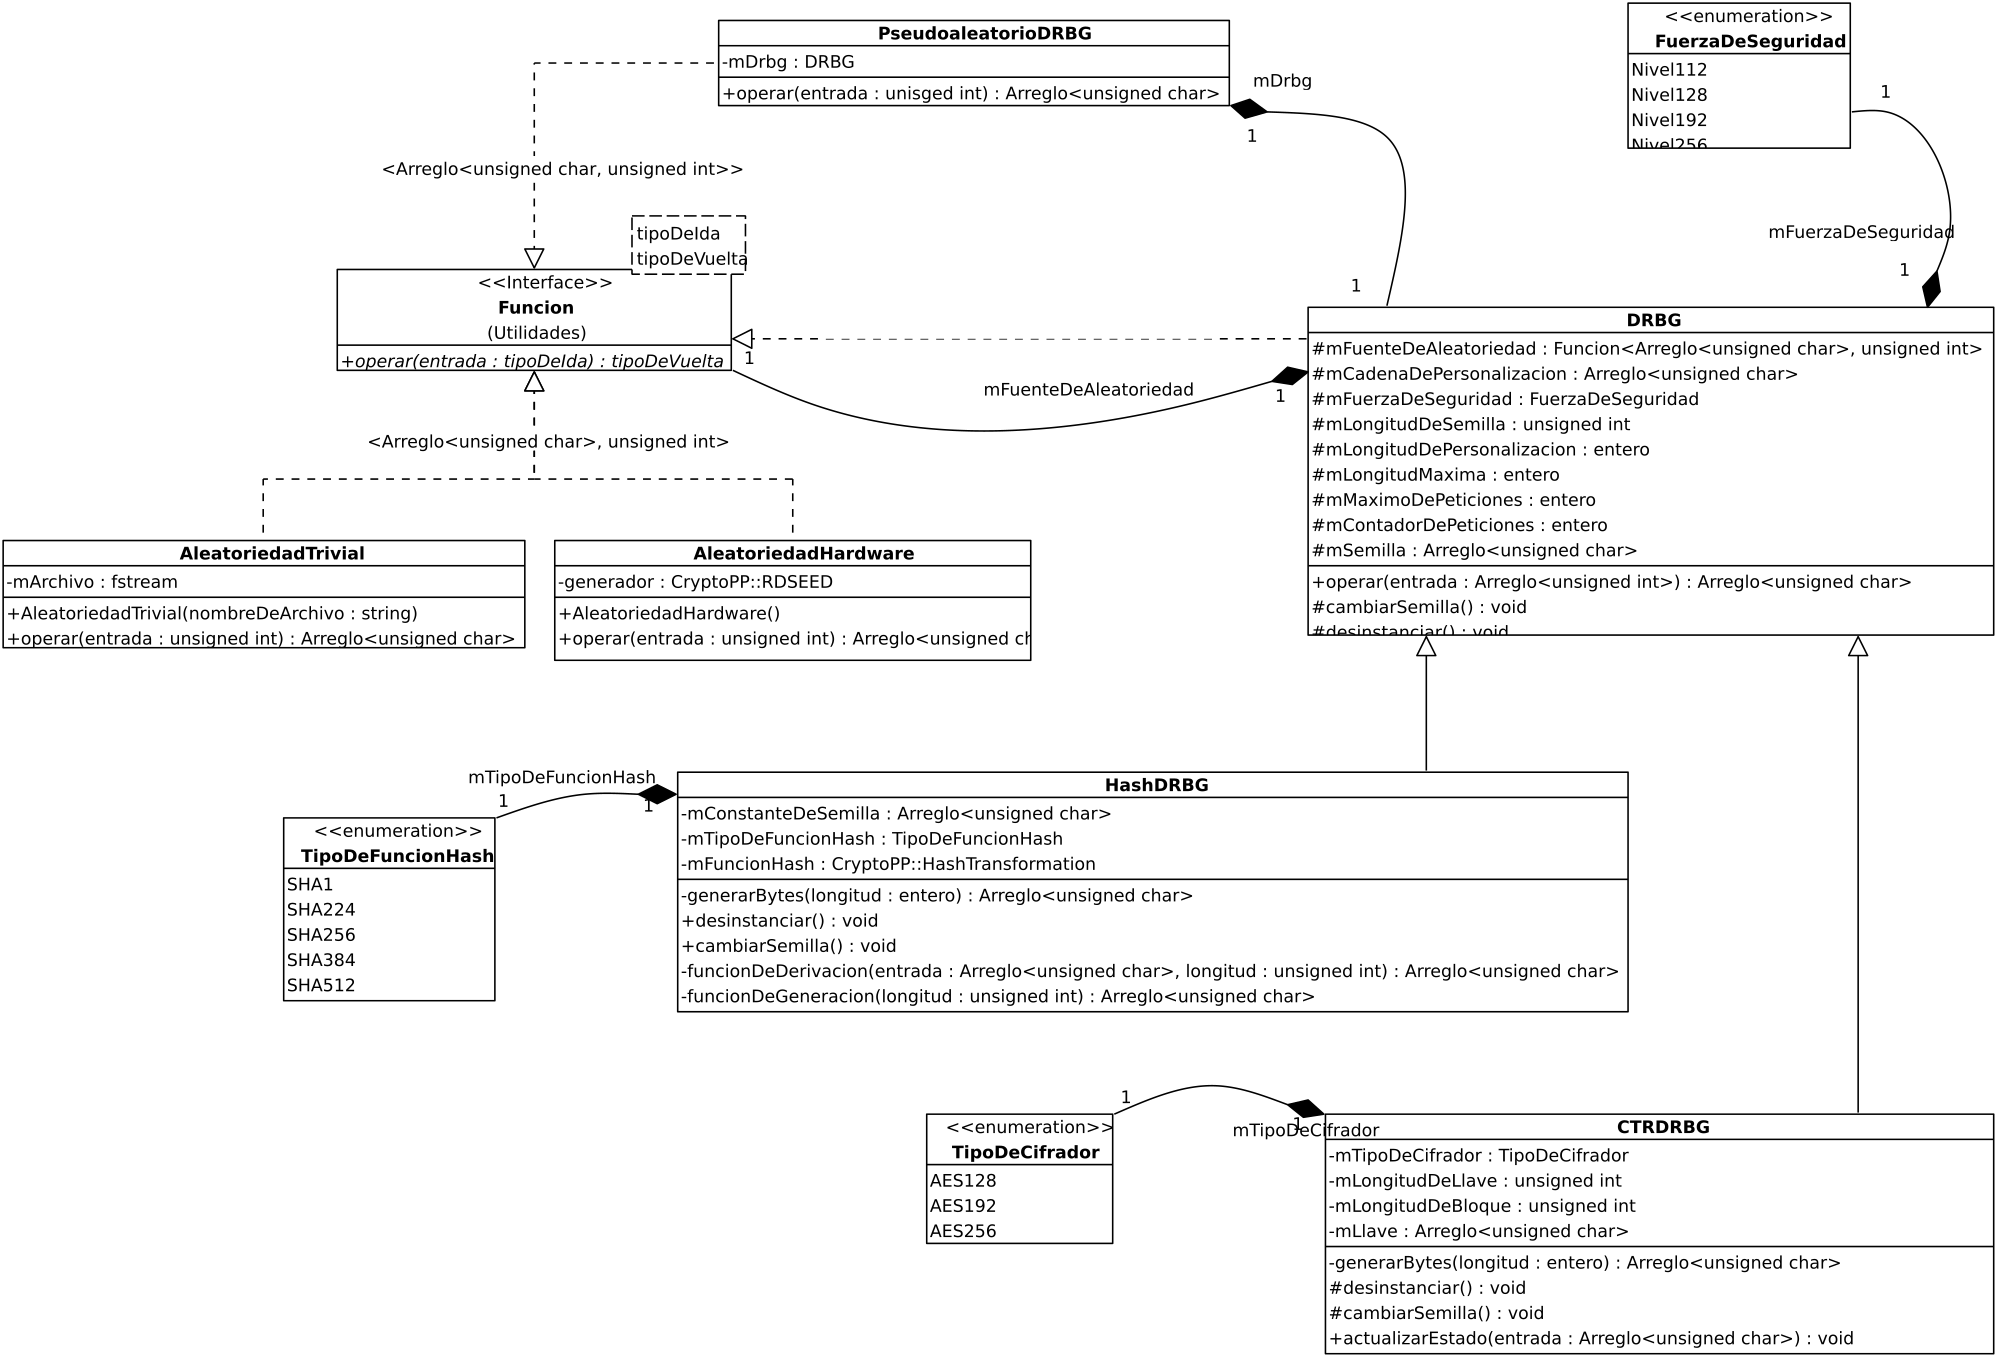
\includegraphics[width=0.8\linewidth]{diagramas/drbg.png}
    \caption{Diagrama de clases de módulo de DRBG.}
    \label{clases_drbg}
  \end{center}
\end{sidewaysfigure}
